A first we are going to introduce the fragment of well-designed SPARQL, then we
will analyze the results of~\cite{pichler2014containment}, in three seperate
chapters namely decidable containment, undecidable containment and equivalence.

\section{Introduction to well-designed SPARQL}
Well-designed SPARQL is a good fundamental basis for complexity analysis because
the evaluation problem is only coNP-complete in contrast to general SPARQL where
it is PSPACE-complete~\cite{perez2009semantics}.
%dbpeda query amount 

\begin{definition}[Well-designed SPARQL]
	A graph pattern $P$ built only from AND and OPT is well-designed if there does
	not exist a subpattern $P' = (P_1 \  \mbox{OPT} \ P_2)$ of $P$ and a variable $?X \in
	vars(P_2)$ that occurs in $P$ outside $P'$, but not in $P_1$. A graph pattern $P
	= P_1 \mbox{ UNION } \dots \mbox{ UNION } P_n$ is well-designed if each subpattern $P_i$ is UNION
	free and well-designed.
\end{definition}

In \cite{letelier2013static} it was shown that every well-designed graph pattern
can be transformed into OPT normal form in polynomial time. 
\begin{definition}[OPT normal form]
	A graph pattern containing only the operators AND and OPT is in OPT normal form
	if the OPT operator never occurs in the scope of an AND operator. 
\end{definition}

Graph Patterns in OPT normal form can be displayed in a natural tree representation, 
formalized by so-called well-designed pattern trees. But before defining the
well-designed pattern trees we need some basic notation about pattern trees.
\begin{definition}[Pattern Tree]\label{def:pt}
	A pattern tree (PT) $T$ is a pair $(T,P)$ where  $T= (V,E,r)$ is a rooted,
	unordered tree and $P = (P_n)_{n \in V}$ is a labelling of the nodes in $V$,
	s.t. $P_n$ is a non-empty set of triple patterns for every $n \in V$.  
\end{definition}

In Example~\ref{ex:pt} we can see how a pattern in OPT normal form is
transformed into a pattern tree.
\begin{example}[~\cite{pichler2014containment}]\label{ex:pt}
	Consider the graph pattern
	\begin{align*}
		P = \big(\big( (x,name,y) \AND (x,email,z) \big) \OPT (x,web,x') \big)
		\OPT \big((x,phone,x'') \OPT (x,fax,x''')\big)
	\end{align*} and the corresponding pattern tree:\\
	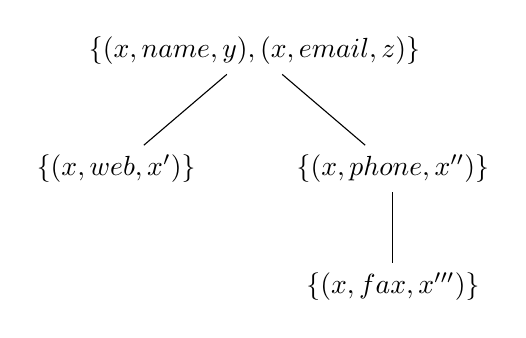
\begin{tikzpicture}[sibling distance=10em]
			\node {\{$(x,name,y),(x, email, z)$\}}
			child { node {$\{(x,web,x')\}$} }
			child { node {$\{(x,phone,x'')\}$}
		child { node {$\{(x,fax,x''')\}$}}};
		\end{tikzpicture}
\end{example}

We will now define further details of a pattern tree and after that
proceed with defining well-designed pattern trees.
\begin{definition}[Components of a pattern tree~\cite{pichler2014containment}]
Let $T = ((V,E,r), P)$ be a pattern tree.

We call the pattern tree $T' = ((V',E',r'), (P_n)_{n \in V'})$ a subtree of $T$
if $(V',E',r')$ is a subtree of $T$. 

An extension of $\hat{T}'$ of a subtree
$T'$ of $T$ is a subtree $\hat{T}'$ of $T$, s.t. $T'$ is in turn a subtree of
$\hat{T}'$. A subtree or extension is proper if some node of the bigger tree is
missing in the smaller tree.

Given $T$, we write $V(T)$ to denote the set $V$ of vertices.

We denote with $pat(T)$ the set $\bigcup_{n\in V(T)} P_n$ and write $vars(T)$ as an
abbreviation for $vars(pat(T))$.

Given a node $n \in V(T)$, we define $branch(n) = n^1, \dots, n^k$ with $n^1 = r$
and $n^k = n$ as the unique sequence of nodes from the root $r$ to $n$.

For nodes $n,\hat{n} \in V(T)$,s.t. $\hat{n}$ is the parent of $n$, let
$newvars(n) = vars(n) \backslash vars(branch(\hat{n}))$. 

A node $n$ is a child
of a PT $T$ if $n\notin V(T)$ and $n$ is the child of some node $n' \in V(T)$.
\end{definition}
After thoroughly describing special details of pattern trees, we are now ready
to look at the definition of well-designed pattern trees(wdPTs).
\begin{definition}[Well-designed pattern tree
	(wdPT)~\cite{pichler2014containment}]
	A well-designed pattern tree (wdPT) is a pattern tree $T = (T,P)$ where for
	every variable $x \in V(T)$, the nodes $\{n \in V(T) \mid x \in vars(n)\}$
	induce a connected subgraph of $T$.
\end{definition}
We can observe that the pattern tree in Example~\ref{ex:pt} is well-designed.
There are two important properties of wdPTs that need to be mentioned. 
\begin{proposition}
	\begin{enumerate}	
		\item Every wdPT $T$ can be transformed efficiently into NR normal form, if $newvars(n) \neq
			\emptyset$ for every $n \in V(T)$~\cite{letelier2012static}. From now on we
			assume w.l.o.g. that all wdPTs dealth with in this paper are in NR normal form.
		\item For every variable $x \in vars (T)$, there is a unique node $n \in
			V(T)$, s.t. $x \in newvars(n)$ and all other nodes $n' \in V(T)$
			with $x \in vars(n')$ are descendants of
			$n$.~\cite{pichler2014containment}
	\end{enumerate}
\end{proposition}


We denote the results of evaluating a wdPT $T$ over some RDF graph by $\ll T
\rr_G$. The set $\ll T \rr_G$ of solutions can be defined via a translation to
graph patterns. We will do something similar in our alternate Definition of
wdPT\ref{def:wdpt}. Lemma~\ref{lemma:altsemwdpt} allows us to use a direct
characterization in terms of maximal subtrees of a wdPT $T$ assuming it is in NR
normal form.
\begin{lemma}[Semantics of pattern trees~\cite{letelier2012static}]\label{lemma:altsemwdpt}
	Let $T$ be a wdPT in NR normal form and $G$ an RDF graph. then $\mu \in
	\ll T\rr_G$ iff there exists a subtree $T'$ of $T$, s.t. 
	\begin{enumerate}
		\item  $dom(\mu) = vars(T')$, and
		\item $T'$ is the maximal subtree of $T$, s.t. $\mu \sqsubset \ll
			pat(T') \rr_G$.
	\end{enumerate}
\end{lemma}

Projection is interpretet as a top level operator on top of a graph pattern.
\begin{definition}[Projection of a mapping]
For a mapping $\mu$ and a set $X$ of variables we denote $\mu_{|X}$ as the
projectino of $\mu$ to the variables in $X$, call it $\mu'$. $dom(\mu'):=X \cap
dom(\mu)$ and $\mu'(x) := \mu(x)$ for all $x \in dom(\mu')$.
\end{definition}

We are now ready to define projected well-designed trees:
A projected well-designed tree (pwdPT) is a pair $(T,X)$ where $T$ is a wdPT and
$X$ a set of variables.
\begin{definition}[Result of pwdPTs \cite{pichler2014containment}]
Let $G$ be a RDF graph. 
Then $\ll (T,X)\rr_G = \{ \mu_{|X} \mid \mu \in \ll T \rr_G\}$.
\end{definition}

In a projected wdPT there are free variables and existential variables.
\begin{definition}[Free and existentail variables
	~\cite{pichler2014containment}]
	Let $(T,X)$ be a pwdPT. Then the free variables of $(T,X)$ are defined as
	$fvars(T)= vars(T) \cap X$ and
	the existential variables of $(T,X)$ are defined as $vars(T) \backslash
	fvars(T)$.
	Analogously, we write $fvars(n)$ and $evars(n)$, respecitvely, for nodes
	$n\in V(T)$.
\end{definition}

In $\cite{letelier2013static}$ it was shown that a 
similar characterization of solution as in Lemma~\ref{lemma:altsemwdpt} exists.
A pwdPT $(T,X)$ is in NR normal form if $T$ is. W.l.o.g., we assume that
existential variables when we look at more than one pwdPT are always renamed apart.

\begin{lemma}[\cite{letelier2013static}]
	Let $(T,X)$ be a pwdPT in $NR$ normal form, $G$ an RDF graph and $\mu$ a
	mapping with $dom(\mu) \subseteq X$. Then $\mu \in \ll ( T,X)\rr_G$ iff
	there exists a subtree $T'$ of $T$, s.t. 
	\begin{enumerate}
		\item $dom(\mu) = fvars(T')$ and
		\item there exists a mapping $\lambda: evars(T') \mapsto dom(G)$, s.t.
			$\mu \cup \lambda \in \ll T \rr_G$.

	\end{enumerate}
\end{lemma}

The last outgrowth of pwdPTs we will consider are unions of well-designed
pattern trees. Unions of well-design patterns correspond to the usage of the
UNION operator in a graph pattern consisting over several well-designed graph
patterns connected by UNION, i.e. $P = P_1 \UNION \dots \UNION P_k$. They can be
considered as a set $\{T_1, \dots, T_k\}$ of wdPTs. Such a set is called
well-designed pattern forest (wdPF) $F$. We can analogously define projected
well-designed pattern forests (pwdPFs) as a tuple $(F',X)$ where $F'=\{(T_1,X),\dots,(T_k,X)\}$.

\begin{definition}[Result of wdPFs and pwdPF \cite{pichler2014containment}]
Let $G$ be a RDF graph. 
Then $\ll F \rr_G = \bigcup_{T\in F}\ll T \rr_G$ and $\ll(F',X)\rr_G =
\bigcup_{(T,X) \in F'} \ll (T,X) \rr_G$. 
\end{definition}


A subforest of a forest $F$ is a set of subtrees of $F$.
We can extend $pat(\cdot)$ to wdPFs: Let $F$ be a wdPF then $pat(F) =
\cup_{T \in F}  pat(T)$ and analogously $vars(F)$.

\bigskip \noindent
To capture the UNION operator the definition of well designed pattern trees
need to be modified.  

Pichler and Skritek studied query containment and query equivalence of well
designed SPARQL in~\cite{pichler2014containment}. As we want to analyse the
complexity of the SERVICE-operator regarding containment and equivalence it 
is crucial to understand the work that was previously done regarding other
SPARQL operators.
Research in query containment and query equivalence is very important in the
context of static query analysis and optimization: Optimization of queries can
be done by replacing a query with a new query which posesses better computational properties. 
Replacing queries
preserving the meaning of the original meaning can only be done by checking if
the replaced query is equivalent to the original query. Also, later on in
Chapter~\ref{chapter:serviceeval}, when we analyse
boundedness of the destination variable of the service operator, we will see
that equivalence plays a role whether a query is feasible to be
evaluated. 
Pichler and Skritek did a fine grained analysis of well-designed SPARQL by
dividing it into several fragments. The fragments are distinguished by
the operators used. All fragments contain triple patterns and the AND-operator. This
fragment corresponds to conjunctive queries which was proven in~\cite{letelier2013static} 
and is denoted with $\{\emptyset\}$. Adding the UNION-operator yields the fragment 
denoted by $\{\cup\}$. Adding projection yields the fragment denoted by $\{\pi\}$ 
and adding both the UNION-operator and projection yields the fragment denoted by $\{\pi,\cup\}$.

In order to define the problems \textbf{CONTAINMENT}, \textbf{EQUIVALENCE} and
\textbf{SUBSUMPTION} which we will investigate on the fragments that we
mentioned above, we need to define what containment, equivalence and subsumption mean
in the SPARQL language.
\begin{definition}[Containment]
\medskip\noindent $P_1$ is contained in $P_2$ $(P_1 \subseteq P_2)$ 
if $\ll P_1 \rr_G \subseteq
\ll P_2 \rr_G$ for every RDF Graph $G$.
\end{definition}
If a graph pattern $P_1$ is contained by a graph pattern $P_2$, all
solutions of $P_1$ are solutions of $P_2$ regardless of the graph
they are evaluated over.

\begin{definition}[Equivalence]
Given two graph patterns $P_1$ and $P_2$ they are equivalent (written as $P_1
\equiv P_2$) if ($\ll P_1 \rr_{G}  = \ll P_2 \rr_{G} $ for every RDF Graph $G$).
\end{definition}
 Equivalence between two graph patterns $P_1,P_2$ means that regardless of the graph
 they get evaluated over, they always have the same solutions.

\begin{definition}[Subsumption]
\medskip\noindent $P_1$ is subsumed by $P_2$ (denoted $P_1 \sqsubseteq P_2$ if for every $\mu \in \ll P_1 \rr_G$ there exists a $\mu' \in
\ll P_2 \rr_G$, s.t. $\mu \sqsubseteq \mu'$. 
\end{definition}
If a graph pattern $P_1$ is subsumed by the graph pattern $P_2$ all the
solutions of $P_1$ can be extended to a solution of $P_2$. This means that if we
add additional mappings to a solution of $P_1$ we can ``build'' a solution of
$P_2$. 


\noindent After reading the definitions of containment, equivalence and
subsumption the following complexity theoretical problems arise:\\
\begin{framed}\noindent CONTAINMENT[$S_1,S_2$]\\
	INPUT: Graph pattern $P_1$ from wd-SPARQL$[S_1]$,
		 graph pattern $P_2$ from wd-SPARQL$[S_2]$\\
	QUESTION: Does $P_1 \subseteq P_2$ hold?
\end{framed}
\begin{framed}\noindent EQUIVALENCE[$S_1,S_2$]\\
	INPUT: Graph pattern $P_1$ from wd-SPARQL$[S_1]$,
		 graph pattern $P_2$ from wd-SPARQL$[S_2]$\\
	QUESTION: Does $P_1 \equiv P_2$ hold?
\end{framed}
\begin{framed}\noindent SUBSUMPTION[$S_1,S_2$]\\
	INPUT: Graph pattern $P_1$ from wd-SPARQL$[S_1]$,
		 graph pattern $P_2$ from wd-SPARQL$[S_2]$\\
	QUESTION: Does $P_1 \sqsubseteq P_2$ hold?
\end{framed}
$S_1$ and $S_2$ always denote a fragment of well-designed SPARQL for example
$\{\cup,\pi\}$. The main results of~\cite{pichler2014containment} are the
solutions to CONTAINMENT[$S_1,S_2$] and EQUIVALENCE[$S_1,S_2$] where $S_1,S_2$
are any of the well designed sparql SPARQL fragments mentioned before.
The results are best represented by the two
tables~\ref{conttable} and~\ref{equivtable}.

\begin{table}
	\begin{minipage}[b]{0.5\hsize}
		\begin{tabular}{|l | l | l | l | l|}
			\hline
			$\downarrow S_1 \backslash S_2 \rightarrow$ & $\{\emptyset\}$  &
			$\{\cup\}$& $\{\pi \}$ & $\{\cup,\pi \}$ \\
			\hline
			$\{\emptyset\}$           & NP-c.	& $\Pi^P_2-c.$  & undec. & undec. \\
			$\{\pi \}$       & NP-c.	& $\Pi^P_2-c.$  & undec. & undec. \\
			$\{\cup \}$      & NP-c.	& $\Pi^P_2-c.$  & undec. & undec. \\
			$\{\cup,\pi \}$ & NP-c.	& $\Pi^P_2-c.$  & undec. & undec. \\
			\hline
		\end{tabular}
		\caption{Containment[$S_1,S_2$]~\cite{pichler2014containment}}
		\label{conttable}
	\end{minipage}
\end{table}

\bigskip
\begin{table}
	\begin{minipage}[b]{0.5\hsize}
\begin{tabular}{|l |  l | l | l | l|}
	\hline
	$\downarrow S_1 \backslash S_2 \rightarrow$ & $\{\emptyset\}$ &
	$\{\cup\}$& $\{\pi \}$ & $\{\cup,\pi \}$ \\
	\hline
	$\{\emptyset\}$			&  NP-c.				& -				 & -         & - \\
	$\{\pi \}$		&  $\Pi^P_2-c.$ 		& $\Pi^P_2-c.$   & -		 & - \\
	$\{\cup \}$		&  $\Pi^P_2-c.$ 		& $\Pi^P_2-h.$   & undec.    & - \\
	$\{\cup,\pi \}$&  $\Pi^P_2-c.$ 		& undec.         & undec.    & undec. \\
\hline
\end{tabular}
\captionof{table}{Equivalence[$S_1,S_2$]~\cite{pichler2014containment}}
\label{equivtable}
	\end{minipage}
\end{table}


\section{Decidable Containment}\label{section:decidablecontainment}

First the decidable cases of Table~\ref{conttable} are proven, i.e., $S_1$ is an arbitrary subsetset of
$\{\cup,\pi\}$ and $S_2$ doesn't contain $\pi$. 
In order to minimize the number of proofs a well known strategy is applied: When membership of a
general case is shown, the more specific case is implied and when showing
hardness for a more specific case, the more general cases are implied.  
Showing the following results fill up the first two columns of the
Containment[$S_1,S_2$] table:
\begin{itemize}
	\item NP-membership of \textbf{CONTAINMENT[$\{\cup,\pi\},\emptyset$]}
	\item $\Pi^P_2$-membership of \textbf{CONTAINMENT[$\{\cup,\pi\},\{\cup\}$]}
	\item $\Pi^P_2$-hardness of \textbf{CONTAINMENT[$\emptyset,\{\cup\}$]}
\end{itemize}
NP-hardness of \textbf{CONTAINMENT[$\emptyset,\emptyset$]} follows immediately
from the NP-hardness of \textbf{EQUIVALENCE[$\emptyset,\emptyset$]} which was shown
in~\cite{letelier2013static}.

For the NP-membership of \textbf{CONTAINMENT[$\{\cup,\pi \}, \emptyset$]}, 
first \textbf{CONTAINMENT[$\{\pi\} , \emptyset$]} is shown and extended to 
\textbf{CONTAINMENT[$\{\cup,\pi \}, \emptyset$]}. We notice that we deal with
both pwdPTs and wdPTs as $S_1$ contains projection. Theorem~\ref{projwd} provides a
necessary and sufficient criterion to decide $(T_1,X) \subseteq T_2$.

\begin{theorem}\label{projwd}\cite{pichler2014containment}
	Let $(T_1,X)$ be a pwdPT and let $T_2$ be a wdPT. Then $(T_1,X) \subseteq
	T_2$ iff for every subtree $T_1'$ of $T_1$,
	\begin{enumerate}
		\item either there exists a child node $n$ of $T_1'$ and a homomorphism
			$h:pat(n) \rightarrow pat(T_1')$ with $h(x) = x$ for all $x \in
			vars(n) \cap vars(T_1')$,
		\item or there exists a subtree $T_2'$ of $T_2$, s.t.
			\begin{enumerate}
				\item $fvars(T_1') = vars(T_2')$
				\item $pat(T_2') \subseteq pat(T_1')$, and
				\item for all extensions $\hat{T_2'}$ of $T'_2$ there exists an
					extension $\hat{T_1'}$ of $T_1'$ and a homomorphism 
					$h: pat(\hat{T_1'}) \mapsto pat(T_1') \cup pat(\hat{T_2'})$
					with $h(x) = x$ for all $x \in vars (T_1')$.
			\end{enumerate}
	\end{enumerate}
\end{theorem}
\begin{proofidea}
Let $G$ be an arbitrary RDF graph. Let $T_1'$ be an arbitrary subtree
of $T_1$. Let $\sigma$ be a mapping s.t. $dom(\sigma) = vars(T_1')$ and $\sigma
\in \ll T_1 \rr_G$. We need to show that $\sigma_{|X} \in \ll T_2 \rr_G$.

The first case of the theorem captures the case where we have a subtree which is
not maximal. For this subtree we could take any $\sigma
\in \ll T_1' \rr_G$ and extend it with the variables in $n$ because  
$h:pat(n) \rightarrow pat(T_1')$ with $h(x) = x$ for all $x \in
vars(n) \cap vars(T_1')$ holds. But such a mapping $\sigma$ can not be in $\ll
T_1 \rr_G$. Thus the subset relation is obviously fulfilled.

The second case captures solutions $\sigma$ with $dom(\sigma) = vars(T'_1)$.
It remains to check if $\mu = \sigma_{|X}$ is in $\ll T_2\rr_G$.
The first two conditions make sure that $\mu$ also maps $T'_2$ into $G$. To make
it a solution for $T_2$ it remains to show that there is no extension $\mu'$ of $\mu$
so that $\mu' \in \ll T_2\rr_G$. Property (2c) makes sure that if $\mu'$ exists,
we can find an extension $\sigma'$ such that it binds more variables than
$\sigma$. But then $\sigma$ is no solution.
\end{proofidea}

To get a better picture of the procedure consider
Example~\ref{ex:membershipcuppiempty}.
\begin{example}[\cite{pichler2014containment}]\label{ex:membershipcuppiempty}
	Assume a $pwdPT(T_1,X)$ with $X = \{x_1, x_2, x_3\}$ and wdPT $T_2$ as
	shown below.

	\bigskip\noindent
	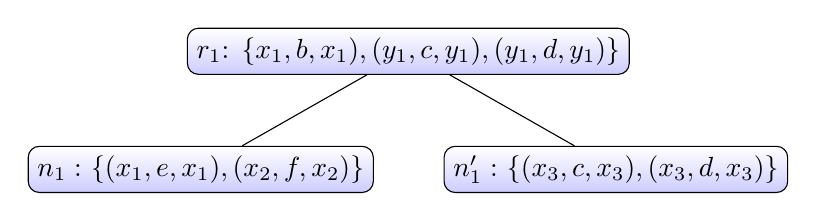
\begin{tikzpicture}[sibling distance=15em,
			every node/.style = {shape=rectangle, rounded corners,
				draw, align=center,
	top color=white, bottom color=blue!20}]]
	\node {$r_1$: $\{x_1,b,x_1),(y_1,c,y_1),(y_1,d,y_1)\}$}
	child { node {$n_1:$ $\{(x_1,e,x_1), (x_2,f,x_2)\}$}}
	child { node {$n'_1:$ $\{(x_3,c,x_3), (x_3,d,x_3)\}$}};
\end{tikzpicture}	

	\bigskip\noindent
	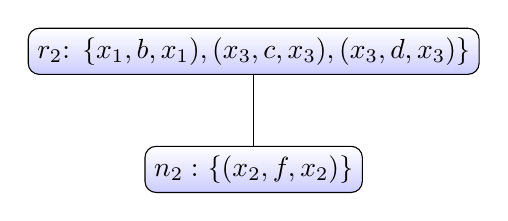
\begin{tikzpicture}[sibling distance=15em,
			every node/.style = {shape=rectangle, rounded corners,
				draw, align=center,
	top color=white, bottom color=blue!20}]]
	\node {$r_2$: $\{x_1,b,x_1),(x_3,c,x_3),(x_3,d,x_3)\}$}
	child { node {$n_2:$ $\{(x_2,f,x_2)\}$}};
\end{tikzpicture}	

\bigskip\noindent
We will now use the criteria in Theorem~\ref{projwd} to check if $(T_1,X) \subseteq T_2$ holds.
Consider all the subtrees of $T_1$: $\{r_1\}, \{r_1,n_1\}, \{r_1,n'_1\}, \{r_1,n_1,n'_1\}$ and check if either of the two properties in Theorem~\ref{projwd} hold.
Consider the subtree $\{r_1, n'_1\}$ and property (2):
We can easily see that the properties (2a) and (2b) are satisfied by the subtree of $T_2$ that contains only 
$r_2$. It remains to check (2c) and this is where the problem occurs:
The required homomorphism from $pat(n_1)$ into $pat(r_1) \cup pat(n'_1) \cup
pat(r_2) \cup pat(n_2)$.
We can also provide the following counterexample:
$G = \{ (g_{x1},b,g_{x1}), (h_{y1},c,h_{y1}),(h_{y1},d,h_{y1}), (j_{x2},f,j_{x2})\}$. Clearly
$\mu \cup \lambda \in \ll T_1 \rr_g$ for $\mu (x_1) = g_{x1}, \mu (x_3) =
h_{y1}$ and $\lambda(y_1) = h_{y1}$ and thus $\mu \in \ll(T_1,X)\rr_G$. However
$\mu \not\in \ll T_2 \rr_G$ because $\mu'$ an extension of $\mu$ can be created
with $\mu'(x_2)=j_{x2}$ and $\mu'(pat(n_2)) \subseteq G$ and thus $(T_1, x)
\not\subseteq T_2$.
We could change $pat(n_2)$ to get $(T_1, x)
\subseteq T_2$: Let $pat(n_2) = \{(x_2,f,x_2,x_1,e,x_1)\}$ and observe that a
homomorphism $h$ for property (2c) of Theorem~\ref{projwd} exists if we define
$h$ as the identity. In fact, then $(T_1,X) \subseteq T_2$.
\end{example}

It is easy to see that Theorem~\ref{projwd} can be transformed into a
$\Pi^P_2$-algorithm: All subtrees $T_1'$ of $T_1$ are tested if there
exists a subtree $T_2'$ of $T_2$ which produces the same mappings as $T_1'$.
On the other hand it is far from obvious, 
that the problem is not $\Pi^P_2$ hard: One can in fact
get rid of one source of complexity and push the complexity of the
\textbf{CONTAINMENT[$\{\pi\},\emptyset$]} problem down to
NP-completeness.
The crucial idea is, that we don't need to look at all the subtrees $T_1'$ of
$T_1$ but polynomially many. The subtrees of interest can be described by
defining the closure of a variable.

It is easy to test if $vars(T_2) = fvars(T_1)$ by traversing the trees once, so
we assume w.l.o.g. that this property holds. Also, we know that $vars(T_2) =
fvars(T_1)$ must hold for $(T_1,X) \subseteq T_2$ to be true as this is an
immediate consequence from Theorem~\ref{projwd} (just consider $T_1' = T_1$).

\begin{definition}[Closure $(C_1(x),C_2(x))$ of a
	variable~\cite{pichler2014containment}]
	Let $(T_1,X)$ be a pwdPT and let $T_2$ be a wdPT with
	$vars(T_2) = fvars(T_1)$. Consider $x \in fvars(T_1)$. The closure
	of $x$ in $(T_1,X)$ and $T_2$ is the pair $(C_1(x),C_2(x))$ where
	$C_i(x)$ (for $i \in \{1,2\}$) is a subtree of $T_i$ such that the
	following conditions are met:
	\begin{enumerate}
		\item $branch(\mbox{new-node}_{T_1}(x)) \subseteq V(C_1(x))$,
		\item $r_2 \in V(C_2(x))$,
		\item $fvars(C_1(x)) = vars(C_2(x))$, and
		\item $C_1(x)$ and $C_2(x)$ are minimal with regard to properties 1-3.
	\end{enumerate}
	Minimality in (4) means that for all subtrees $D_1$ of $T_1$ and $D_2$ of
	$T_2$, if $D_1$ and $D_2$ satisfy conditions 1-3, then $V(C_1) \subseteq
	V(D_1)$ and $V(C_2) \subseteq V(D_2)$ meaning the nodes for the subtrees
	$V(C_1)$ and $V(C_2)$ are minimized.
\end{definition}

Because we assumed $vars(T_2) = fvars(T_1)$ we can easily see that the closure
always exists. 

\begin{proposition}[~\cite{pichler2014containment}]
	Let $(T_1,X)$ be a pwdPT and let $T_2$ be a wdPT with $fvars(T_1) =
	vars(T_2)$. Then the closure $(C_1(x),C_2(x))$ exists and can be
	efficiently computed.
\end{proposition}
\begin{proofidea}
	The algorithm chooses a not yet chosen variable $x \in fvars(T_1)$ and
	initializes the trees $C_1(x)$ and $C_2(x)$ by setting $C_1(x) =
	\mbox{branch}(\mbox{new-node}_{T_1})$ and $C_2(x) = V(C_2(x)) = \{r_2\}$ where $r_2$ is
	the root of $T_2$. It remains to fulfill the condition $fvars(C_1(x)) =
	vars(C_2(x))$ in such a way that $C_1(X)$ and $C_2(X)$ are minimal with
	regard to the number of vertices. We either have one of the following cases:
	\begin{enumerate}
		\item $fvars(C_1(x)) = vars(C_2(x))$: This means we are done and have
			successfully computed the closure $(C_1(x), C_2(x))$
		\item $fvars(C_1(x)) \supset vars(C_2(x))$: This means we miss the
			variables\\ $fvars(C_1(x)) \backslash vars(C_2(x))$. By
			iteratively adding $\mbox{branch}(\mbox{new-node}_{T_2}(y))$ to $C_2(x)$ for all
			variables\\ $y \in fvars(C_1(x)) \backslash vars(C_2(x))$ all
			the missing variables are now in $C_2(x)$.
		\item $fvars(C_1(x)) \subset vars(C_2(x))$: This means we miss the
			variables\\ $vars(C_2(x)) \backslash fvars(C_1(x))$. By iteratively
			adding $\mbox{branch}(\mbox{new-node}_{T_1}(y))$ to $C_1(x)$ for all variables
			$y \in vars(C_2(x)) \backslash fvars(C_1(x))$, all the missing
			variables are now in $C_1(x)$.
	\end{enumerate}
	By the assumed condition $fvars(T_1) = vars(T_2)$, the procedure will
	eventually reach a fixpoint~\cite{pichler2014containment}.
\end{proofidea}

Using the closure of the variable is inspired by the following idea:
Assume $\mu$ is a solution mapping of $(T_1,X)$ and $y$ is part of $\mu$, i.e.,
a free variable. Now we need to show that $\mu$ is also part of $T_2$, i.e.,
$\mu$ must bind all the variables that occur in $T_2$ on the branch from the
root to the node $n$ where $y$ is introduced. If again an additional variable
$z$ is introduced in this path in tree of $T_2$, $\mu$ must bind all the free
variables in $(T_1,X)$ along the branch from the root to the first occurrence of
$z$. Using the idea of the closure allows us to formulate an alternative characterization of
$(T_1,X) \subseteq T_2$. The improvement is that we only need to check
polynomially many closures and not exponentially many subtrees of $(T_1,X)$.

\begin{theorem}[\cite{pichler2014containment}]\label{projwd2}
	Let $(T_1,X)$ be a pwdPT and let $T_2$ be a wdPT. Then $(T_1,X) \subseteq
	T_2$ if and only if $fvars(T_1) = vars(T_2)$ and for every $x \in
	fvars(T_1)$
	\begin{enumerate}
		\item $pat(C_2(x)) \subseteq pat(C_1(x))$
		\item for every $n \in V(C_1(x)) \ \mbox{branch} (\mbox{new-node}_{T_1}(x))$, there
			exists a homomorphism $h_1: pat(n) \mapsto pat(\mbox{branch}(\hat{n})) \cup
			pat(\mbox{branch}(\mbox{new-node}_{T_1}(x)))$ (where $\hat{n}$ is the parent node
			of n in $T_1$) with $h_1(x) = x$ for all $x \in vars(n) \cap
			(vars(branch(\cap{n})) \cup vars(\mbox{branch}(\mbox{new-node}_{T_1}(x))))$, and
		\item for every child node $m$ of $C_2(x)$, and for every variable $y
			\in newvars(m)$, the following property holds: let $n \in
			\mbox{branch}(\mbox{new-node}_{T_1}(y))$. Then there exists a homomorphism
			$h_2:pat(n) \mapsto pat(C_1(x)) \cup pat(m) \cup
			pat(\mbox{branch}(\hat{n}))$ (where $\hat{n}$ is the parent node of $n$)
			with $h_2(x) = x$ for all $x \in vars(n) \cap (vars(C_1(x)) \cup
			vars(\mbox{branch}(\hat{n})))$.
	\end{enumerate}
\end{theorem}
\begin{proofidea}
	The first property is the most obvious one: every mapping $\sigma$ which is
	a solution for $C_1(x)$ assuming $G$ as our arbitrary graph, results in $\mu =
	\sigma_{|X}$ also being a solution for $C_2(x)$.
	The second condition makes sure that when $x$ is in the domain of the
	solution mapping $\sigma$ all of $C_1(x)$ was used when retrieving the
	mapping $\sigma$ from $G$.
	The last condition is similar to the condition (2c) in the
	Theorem\ref{projwd}: When $\mu = \sigma_{|X}$ with $dom(\mu) =
	vars(C_2(x))$ is not a solution for $T_2$ because $C_2(x)$ could have been
	extended with some child of $C_2(x)$ it must be that it is possible to
	extend $\sigma$ to some child of $C_1(x)$.
\end{proofidea}

In the actual proof of Theorem~\ref{projwd2}, Theorem~\ref{projwd} is used to show
that the conditions of Theorem~\ref{projwd2} are also sufficient.

\begin{theorem}[\cite{pichler2014containment}]\label{ccuppiempty}
	CONTAINMENT$[\{\cup,\pi\},\emptyset]$ is in NP.
\end{theorem}
\begin{proof}
	Similarly to Theorem~\ref{projwd} we can construct a procedure using Theorem~\ref{projwd2} 
	which is in NP.
	Let $(F,X)$ be a well designed pattern forest (pwdPF) and let $T$ be a
	$wdPT$. Consider now every pwdPT $F'$ in the forest $(F,X)$ and
	use our procedure to decide $(F',X) \subseteq T$. Put more formally we get $(F,X) \subseteq T$ iff.
	$(T_i,X) \supseteq T$ for every $(T_i,X) \in (F,X)$.
\end{proof}

The next problem that we tackle is \textbf{CONTAINMENT$[\{\cup,\pi\},\{\cup\}]$}: First
a necessary and sufficient condition for containment is given and then turned
into an algorithm. For this formulation the definition of a renamed proper
extension of a wdPF is important.
\begin{definition}[\cite{pichler2014containment}]
	Let $F = \{ T_i \mid \mbox{with } 1\leq i \leq k\}$ be a wdPF, $F'$ a
	subforest of $F$. For every $T_i \in F$, an injective renaming function
	$\rho_i$ with $dom(\rho_i) = vars(T_i)$, s.t. 
	\begin{enumerate}
		\item $\rho_i(x) = x$ for all $x \in vars(F')$,
		\item $\rho(x) \neq \rho(y)$ for every $x \in vars(T_i) \backslash
			vars(F'),i\neq j \in \{ 1, \dots, k\}$ and $y \in dom(\rho_j)$.
			Finally let $\hat{F}$ be the wdPF $\{ \rho_i(T_i) \mid 1 \leq i \leq
			k\}$. 
	\end{enumerate}
	Then a renamed proper extension of $F'$ is a subforest of
	$\hat{F}$, call it $\hat{F}'$ that has $F'$ as a proper subforest, i.e.,
	$\hat{F}'$ is not equal to $F'$.
\end{definition}

\begin{theorem}[\cite{pichler2014containment}]\label{projwd3}
	Let $(T_1,X)$ be a pwdPT and let $F_2$ be a wdPF. Then $(T_1,X) \subseteq
	F_2$ iff for every subtree $T'_1$ of $(T_1,X)$:
	\begin{enumerate}
		\item either there exists a child node $n$ of $T'_1$ s.t. there is a
			homomorphism $h: path(n) \mapsto pat(T'_1)$ with $h(x) = x$ for
			all $x \in varS(n) \cap vars(T_1')$
		\item or there exists a subtree $T'_2$ of $F_2$ with $vars(T'_2) =
			fvars(T_1')$ and $pat(T'_2) \supseteq pat(T'_1)$ s.t. every
			renamed proper extension $F'_2$ of $\{T'_2\}$ in $F_2$ satisfies one
			of the following properties:
			\begin{enumerate}
				\item \label{firstcaseprojwd3}there exists a proper renamed extension $\hat{F}'_2$ of
					$F'_2$ (i.e. a bigger extension than $F'_2$ nodewise),
					and a homomorphism $h_a: pat(\hat{F}'_2) \mapsto
					pat(F'_2)$ with $h(x) = x$ for all $x \in
					vars(\hat{F}'_2)\cap (vars(F'_2) \cup vars(T'_1))$, or
				\item there exists an extension $\hat{T}'_1$ of $T'_1$ and a
					homomorphism $h_b: pat(\hat{T}'_1) \mapsto pat(F_2') \cup
					pat(T'_1)$ with $h(x) =x$ for all $x \in vars(T_1')$, or
				\item case (2a) does not apply and there
					exists a tree $T \in F'_2$ with $vars(T)= fvars(T'_1)$.
			\end{enumerate}
	\end{enumerate}
\end{theorem}
\begin{proofidea}
 The conditions presented in Theorem~\ref{projwd3} are similar to those presented in
 Theorem~$\ref{projwd}$: First we choose an arbitrary subtree $T'_1$ of $(T_1,X)$ and
 inspect the mappings $\sigma$ that $T'_1$ induces assuming an arbitrary Graph
 $G$: 
 \begin{itemize}
	 \item Either $\sigma$ can be extended to some child node of $T_1'$ but then
 again $\sigma$ is not a solution of $(T_1,X)$ over $G$
	 \item  or $\sigma_{|X} \in \ll F_2\rr_G$.
\end{itemize}
Condition (1) takes care of subtrees for which $\sigma$ could be extended
to some additional child node of the subtree. This would mean that the subtree
is not a valid solution for $(T_1,X)$.
Condition (2) extends condition (2) from Theorem\ref{projwd}:
It is easy to see that we fulfill condition (2a) and condition (2b)
from Theorem~\ref{projwd} similarly by saying that the subtree $T'_2$ of $F_2$
with $vars(T'_2) = fvars(T'_1)$ and $pat(T'_2) \subseteq pat(T_1')$.  
The condition(2c) of Theorem~\ref{projwd} was used to make sure
that any extension $\mu'$ of $\mu$ for which $\mu' \in \ll T_2\rr_G$ holds would
result in $\sigma$ being no solution of $T_1$ over $G$. To extend
condition (2c) of Theorem~\ref{projwd} the notion of proper renamed extension
comes into use. This is due to the fact that we now have a pattern forest and
$\mu$ might still be a solution of another tree in $F_2$. This means that all
subtrees in $F_2$ with $vars(T'_2) = fvars(T'_1)$ and $pat(T'_2) \subseteq
pat(T'_1)$ must be eligible to be extended to show that $\mu$ is indeed not a
solution of $F_2$ but extensions of $\mu$ are solutions.
Condition $(2a)$ forces a certain maximality condition onto the proper renamed
extensions of $T'_2$, i.e., we cant have more nodes in the proper renamed
extension $F'_2$ without having a pattern mismatch in the proper renamed
extension $F'_2$ and
the extension $\hat{F}'_2$ of it. A pattern mismatch means that the homomorphism $h_a:
pat(\hat{F}'_2) \mapsto pat(F'_2)$ does not exist.
Condition $(2c)$ makes sure that the proper renamed extension $F'_2$
extends all the relevent subtrees of $F_2$, i.e. a relevant subtree is a tree $T
\in F'_2$ where $vars(T)  =fvars(T'_1)$.
%!!anm: that is not already included into
%the subforest $F'_2$.???!!
Condition (2b) checks for the existence of a homomorphism $h_b$ that maps
$pat(\hat{T'_1})$ into the patterns of the renamed proper extension $pat(F_2)
\cup pat(T_1')$.

\end{proofidea}

\begin{theorem}[\cite{pichler2014containment}]
	CONTAINMENT$[\{\cup,\pi\},\{\cup\}]$ is in $\Pi^P_2$.
\end{theorem}
\begin{proof}
	The characterization in Theorem~\ref{projwd3} yields a more or less
	straightforward $\Sigma^P_2$-algorithm for testing $(T_1,X) \not\subseteq
	F_2$: first guess $T'$ and the proper renamed extension $\hat{F}'_2$, and
	then use a coNP-oracle that there does not exist a child node $n$ and
	homomorphism $h$ as described by property $(2b)$.
	To now show \textbf{CONTAINMENT[$\{\cup,\pi\},\{\cup\}$]} we extend the algorithm
	wdPF in the following way: $(F_1,X) \subseteq F_2$ iff. $(T_i,X) \subseteq
	F_2$ for every $(T_i,X) \in (F_1,X)$.
\end{proof}

The hardness proof of \textbf{CONTAINMENT[$\emptyset,\{\cup\}$]} is done by a reduction from
the well known $\Pi^P_2$-complete problem 3-QSAT$_{\forall,2}$. !!citation.

\begin{framed}\noindent 3-QSAT$_{\forall,2}$\\
	INPUT:A formula $\phi= \forall \vec{x}\exists \vec{y} \psi$,\\
	where $\psi$ is a Boolean formula in CNF over the variables
	$\vec{x}\cup\vec{y}$.
	
	QUESTION: Can every assignment $I$ on the variables in $\vec{x}$ be extended
	to an assignment $J$ on $\vec{y}$, s.t. $J \models \psi$?
\end{framed}


\begin{theorem}[\cite{pichler2014containment}]\label{cemptycup}
	CONTAINMENT$[\emptyset,\{\cup\}]$ is $\Pi^P_2$-hard.
\end{theorem}
\begin{proofidea}
	Assume an arbitrary instance of $3-QSAT_{\forall,2}$ and construct an
	instance of \textbf{CONTAINMENT$[\emptyset,\{\cup\}]$} as follows: The wdPT $T_1$
	consists of the root and two child nodes: $n_i, n'_i$ for every variables
	$x_i \in \vec{x}$. In this way we are able to model the assignment $I$ of
	the 3-QSAT$_{\forall,2}$ problem in form of subtrees of $T_1$. 
	Additionally we have a child node $n_0$ containing the
	variables in $\vec{y}$ and an encoding of the formula $\psi$. 
	
	It remains to deal with the ``unintended'' subtrees of $T_1$ where given an
	$i$ either both $n_i$ and $n'_i$, or neither $n_i$ and $n'_i$ are in the subtree.
	This is done by adding certain wdPTs to $F_2$ which take care of the two
	problems. The last wdPT added to the forest $F_2$ contains the triples
	encoding the formula $\psi$ in its root plus the child nodes $n_i,n'_i$.
	This wdPT produces the solutions of all ``intended'' subtrees of $T'_1$ if
	and only if every assignment $I$ on the variables in $\vec{x}$ can be
	extended to an assignment $J$ on $\vec{y}$, s.t. $J \models \psi$.
\end{proofidea}

The section dealing with decidable containment closes with settling the
complexity of SUBSUMPTION$[S_1,S_2]$ problem for every $S_1, S_2 \subseteq \{
\cup, \pi \}$. In prior work \cite{letelier2012static} it was shown, that the simple case
$S_1=S_2=\emptyset$ is $\Pi_2^P-complete$. 
Later on in~\cite{letelier2013static} the $\Pi^P_2$-membership 
was extended to the case where $S_1 = S_2 = \{\pi\}$ holds.
To establish the $\Pi^P_2$-completeness to arbitrary $S_1,S_2 \subseteq \{ \cup,
\pi \}$, it obviously suffices to show the $\Pi_2^P$-membership for the most general case.

\begin{theorem}[\cite{pichler2014containment}]\label{scuppicuppi}
	\textbf{SUBSUMPTION[$\{\cup,\pi\}, \{ \cup, \pi \}$]} is in $\Pi^P_2$.
\end{theorem}
\begin{proofidea}
	Let $(F_1,X)$ and $(F_2,X)$ be two pwdPFs.
	The main proofidea is that the following critera for subsumption was found:
	$(F_1,X) \sqsubseteq (F_2,X)$ iff for every subtree $T'_1$ of $F_1$, there
	exists a subtree $T'_2$ of $F_2$, s.t.
	\begin{enumerate}
		\item $fvars(T'_1) \subseteq fvars(T'_2)$ and
		\item there exists a homomorphism $h:pat(T'_2) \mapsto pat(T'_1)$
			with $h(x)= x$ for all $x \in fvars(T_1')$.
	\end{enumerate}
	Consider now the following procedure:
	For all subtrees $T'_1$ of $F_1$ check that there exists a subtree $T'_2$ of
	$F_2$ together with a homomorphism of the desired property. This procedure
	can be executed in $\Pi_2^P$ because we have need to check all subtrees
	for a property which would be in co-NP, but then the property is a
	homomorphism check which is in NP. So we have a co-NP$^{\mbox{NP}}$ runtime.
\end{proofidea}

In~\cite{letelier2012static} the authors noticed an interesting feature of
subsumption in SPARQL: In the fragment of wd-SPARQL$[\emptyset]$ subsumption is
able to characterize equivalence. Assume graph patterns $P_1,P_2 \in$
wd-SPARQL[$\emptyset$]. Then $P_1 \equiv P_2$ iff. $P_1 \sqsubseteq P_2$ and 
$P_2 \sqsubseteq P_1$. In~\cite{letelier2013static} the authors were able to
find a counterexample for wd-SPARQL[$\pi$]. 
Now in~\cite{pichler2014containment} the result is strengtened:
Assuming one pattern $P_1$ in wd-SPARQL[$\emptyset$] and one pattern $P_2$ in either
wd-SPARQL[$\{\pi\}$] or wd-SPARQL[$\{\cup\}$] one can show that $P_1 \not\equiv
P_2$ but $P_1 \sqsubseteq P_2$ and $P_2 \sqsubseteq P_1$.

\begin{proposition}[\cite{pichler2014containment}]
	There exist pairs $P_1,P_2$ of graph patterns $P_1$ from
	wd-SPARQL[$\emptyset$] and $P_2$ from either wd-SPARQL[$\{\pi\}$]
	wd-SPARQL[$\{\cup\}$], s.t. $P_1 \sqsubseteq P_2$ and $P_2 \sqsubseteq P_1$
	hold but $P_1 \not\equiv P_2$.
\end{proposition}
\begin{proofidea}
	It is an easy observation that we need two counterexamples to prove the
	proposition. 
	\begin{enumerate}	
		\item At first we consider the case where  $P_1 \in$
			wd-SPARQL[$\emptyset$] and  $P_2 \in$ wd-SPARQL[$\{\cup\}$]. Let
			$P_1 = (t_1 \OPT t_2)$ and $P_2 = ((t_1) \UNION (t_1 \AND t_2))$. The patterns $t_1$ and $t_2$
			are assumed to be distinct.
			$P_1 \sqsubseteq P_2$ can be easily seen because $P_2$ more or less models
			the semantics of $OPT$. $P_2 \sqsubseteq P_1$ Also holds because again the
			semantics of opt are projected into $P_2$. But $P_1 \sqsubseteq P_2$ does
			obviously not hold since $P_2$ always has mappings which are solely created by
			$t_1$.
		\item 
			Now for the second counterexample where  $P_1 \in$
			wd-SPARQL[$\emptyset$] and  $P_2 \in$ wd-SPARQL[$\{\pi\}$]. 
			$P_1 = (x_1,a,x_2) \OPT ((x_3,a,x_2) \AND (x3,a,x_3))$\\
			and
			$P_2 = ((x_1,a,x_2) \AND (y_1,a,Y_2)) \OPT ((x_3,a,x_2) \AND
			(x_3,a,x_3)\\ \AND (y_3,a,y_2) \AND (y_3,a,y_3))$ and $X =
			\{x_1,x_2,x_3\}$.
			It remains to show that $P_1 \sqsubseteq (P_2,X)$ and $(P_2,X)
			\sqsubseteq P_1$ but $P_1 \not\equiv (P_2,X)$.
		    Towards this goal we observe that the triple patterns in $P_1$ are
			contained in $P_2$. Also, $P_2$ contains triple patterns with
			existential variables. We can easily see that there is a
			homomorphism mapping the triple patterns containing the existential
			variables to into the
			patterns of $P_1$. Thus $P_1 \sqsubseteq (P_2,X)$ holds. Also
			$(P_2,X) \sqsubseteq P_1$ holds, but in general $(P_2,X) \not\subseteq
			P_1$ since one can provide a graph $G$ and an appropriate
			instantiation of the existential variables $y_1, y_2$ in the root
			of $P_2$ that block the extension of mapping to the child node.
			Consider the following RDF graph $G = \{ a(1,1), a(2,3)\}$. Then
			$\mu = \{x_1 \mapsto 1, x_2 \mapsto 1\} \in \ll (T_2,X)\rr_G$,
			because of the mapping $\lambda = \mu \cup \{ y_1 \mapsto 2,
			y_2\mapsto 3 \} \in \ll T_2 \rr_G$ which cannot be extended to the
			child node of $r_2$ However $\mu \notin \ll T_1\rr_G$ since $\mu$
			can be extended to the child node of $r_1$ by adding $[x_3 \mapsto
		1]$.
			
	\end{enumerate}
\end{proofidea}

\section{Undecidable Containment}
We can see in table~\ref{conttable} that
\textbf{CONTAINMENT$[S_1,S_2]$} is undecidable, when $\pi \in S_2$. Again we don't need to show
the undecidability for every entry in the table, as we can just show it for the
most specific entry, i.e.,
\textbf{CONTAINMENT[$\emptyset,\{\pi\}$]}. We do this proof by
reducing from the conjunctive query answering problem under integrity 
constraints in form of tuple generating dependencies (abbr. tgds)~\cite{JOHNSON1984167,cali2008taming}. This problem
is well known to be undecidable~\cite{JOHNSON1984167,cali2008taming}. We are not going to reduce the original problem but a modified version of it to our problem. 
Three changes need to be made, to make the problem suitable for us:
\begin{enumerate}
	\item  The undecidability results for the problem refer to arbitrary
		databases, which would include infinite databases. Our RDF graphs
		however are a finite set of triples.
	\item The problem allows predicates of arbitrary length but our RDF graphs
		contains only triples. 
	\item Finally, for the problem reduction in the end, it turns out to be
		convenient to restrict the problem from a set of tgds to a single tgd.
\end{enumerate}

Before doing the first step, it is crucial to define tuple generating dependencies 
and the undecidable problem, namely \textbf{CQ-UNDER-TGDs}.

\begin{definition}[tuple generating dependency]
	Let $\phi(\vec{x})$ and $\psi(\vec{x},\vec{y})$ be conjunctive queries.
	Also, let all variables $\vec{x}$ occur in $\phi(\vec{x})$.
	A tuple generating dependency (tgd) is a first-order formula of the form 
	$\forall \vec{x} (\phi(\vec{x}) \rightarrow \exists \vec{y})
	\psi(\vec{x},\vec{y})$.
\end{definition}
To simplify the notation of a tgd, the $\forall$-quantifiers are omitted.
Let $I$ be a database instance and $\tau$ be a tgd. Then we define $I \models
\tau$ %holds,
%like the usual satisfaction relation for first-order formulas. Another way to
%define satisfaction would be  
using homomorphisms. This is feasible, because a tgd is an implication:
For every homomorphism $h: \phi(\vec{x}) \mapsto I$ (mapping constants to
themselves), which is responsible for the antecedent of the implication, there
must be an extension $h'$ of $h$, for which $h':\psi(\vec{x},\vec{y}) \mapsto I$
holds. It is then natural to define satisfaction for a set of tgds: Let $\Sigma$
be a set of tgds. Then $I \models \Sigma$ iff. $I \models \tau$ for every $\tau
\in \Sigma$.
Let $Q$ be conjunctive query. For a set $\Sigma$ of tgds, a database instance
$I$ and a BCQ $Q$, we say that $I,\Sigma \models Q$ holds, if for every
(possible infinite) database instance $M$, s.t. $M \models \Sigma$ and $I
\subseteq M$, we also have $M \models Q$. We write $I, \Sigma \models_f Q$ if
only finite models $M$ are allowed.

Consider now the two problems:
\begin{framed}\noindent \textbf{CQ-UNDER-TGDs}\\
	INPUT: set $\Sigma$ of tgds, database instance $I$ and a CQ $Q$.\\
	QUESTION: does $\Sigma, I\models Q$ hold? 
\end{framed}
\begin{framed}\noindent \textbf{FINITE-CQ-UNDER-TGDs}\\
	INPUT: set $\Sigma$ of tgds, database instance $I$ and a CQ $Q$.\\
	QUESTION: does $\Sigma, I\models_f Q$ hold? 
\end{framed}
We proceed with step one procedure:
By~\cite{cali2008taming} \textbf{CQ-UNDER-TGDS} is undecidable. The proof
in~\cite{cali2008taming} will be changed so that
\textbf{FINITE-CQ-UNDER-TGDs} remains
undecidable even though $|\Sigma| = 1$.
%Then a reduction from this restricted version of \textbf{FINITE-CQ-UNDER-TGD} to
%\textbf{CONTAINMENT[$\emptyset,\{\pi\}$]} will be produced to establish the sought-after
%result.
Examining the undecidability proof of \textbf{BCQ-UNDER-TGDs} in~\cite{cali2008taming}, 
a reduction from the HALTING problem to \textbf{BCQ-UNDER-TGDs} is given: The
initial configuration of the Turing machine is encoded into the instance $I$ and
several $tgds$ are used to describe the transitions of the $TM$. The query $Q$
descrbes the halting condition.
It is then shown that the Turing Machine halts iff $\Sigma,I \models Q$ holds.
When the machine doesn't halt, one can construct a counter-model $M$ for
$\Sigma,I \models Q$. For this model $M \models \Sigma$ and $I \subseteq M$ but
$M \not \models Q$. This construction is defined by the straightforwards
encoding of the infinite run of the $TM$. 
\begin{proposition}~\cite{pichler2014containment}
	The same reduction cannot work for \textbf{FINITE-CQ-UNDER-TGDs}.
\end{proposition}

\begin{proof}
Proof by contradiction.	
Assume the same reduction works for \textbf{FINITE-CQ-UNDER-TGDs}.
Testing if $I,\Sigma \not\models_f Q$ holds) (the co-problem of
\textbf{FINITE-CQ-UNDER-TGDs}) is semi-decidable:
In a loop enumerate all finite models $M$ and then in the loop check, if $M
\models I$, $M \models \Sigma$ and $M \not\models_f Q$ holds. If we then use the
assumption that the same reduction works, we could reduce from
\textbf{co-CQ-UNDER-TGDs}
to \textbf{co-FINITe-CQ-UNDER-TGDs}. Which would mean \textbf{co-CQ-UNDER-TGDs} is semidecidable.
But asking if $I,\Sigma \models Q$, i.e. \textbf{co-CQ-UNDER-TGDs} is semi-decidable because it is the same as asking for unsatisfiability of the set of FO formulas $I,\Sigma,\not Q$ due to
the semi-decidability of first-order logic. But then the established
undecidability of the halting problem would not halt and we have a
contradiction.
\end{proof}
Even though the proof cannot be used to prove \textbf{FINITE-BCQ-UNDER-TGDs} undecidable
the following theorem was established:

\begin{theorem}\label{fund}~\cite{pichler2014containment}
	\textbf{FINITE-BCQ-UNDER-TGDs} is undecidable.
\end{theorem}
\begin{proofidea}
	The main idea is that \textbf{co-HALTING} is reduced to
	\textbf{FINITE-CQ-UNDER-TGDs}. 
	The initial configuration of the TM is encoded in the instance $I$ and the
	transitions of the TM are encoded by the tgds. 
	The atoms $state(x,q), cursor(x,p)$ and $contains(x,y,s)$ are used to
	represent a configuration of the turing machine. Using the mentioned atoms one can
	express that at some time instant $x$, the TM is in state $q$, the cursor is
	in position $p$ and the tape content of tape cell $y$ is $s$.
	The successor relation $next(x,x')$ is defined that can be applied to time
	instants and tape positions.
	Now back to the adaptions from the original transformation:
	\begin{enumerate}
		\item A relation $smaller(\cdot,\cdot)$ is introduced and
		used to encode the transitive closure of $next(\cdot,\cdot)$.
	\item The query $Q$, remember, this was prior used to encode the halting
			condition, now asks for $smaller(x,x)$, i.e., if there exists some
		``loop'' in the time instants.  
	\end{enumerate}
	$I,\Sigma \models_f Q$ holds iff the TM does not halt can be shown.
	Assuming the TM halts, a simple countermodel $M$ in form of the natural encoding
	of the halting run of the TM can be found.
	Suppose that the TM does not halt. Then every model $M$ of $I,\Sigma$
	contains an encoding of the infinite number of steps in the non-halting run
	of the TM. Now we use our assumption that $M$ is finite and every step is
	identified by some time instant. Thus at least one symbold $a$ is used to
	encode more than one time instant (which results in the loop). Thus
	$smaller(a,a) \in M$. If $smaller(x,x)$ occurs we have a (non-halting) run of the TM. 
	Since each step(state, cursor position and cell content) is identified by
	some time instant and $M$ is finite. 
\end{proofidea}

For completing step two and three of our procedure, we need to strengthen the
undecidability result from~\ref{fund} to atoms with arity two and to restrict
the set of tgds in \textbf{FINITE-CQ-UNDER-TGDs} to a singleton. 
Notice that atoms of arity two are just a different representation of triples. 
$p(s,o) \sim (s,p,o)$.

\begin{theorem}\label{fundplus}~\cite{pichler2014containment}
	\textbf{FINITE-BCQ-UNDER-TGDs} is undecidable, even if the arity of every relation
	symbol is at most two and even if $\Sigma$ consits of a single tgd.
\end{theorem}

\begin{proofidea}
To construct a single tgd $\tau$ from $\Sigma$ all antecedents of the thfd in
$\Sigma$ are combined into one antecedent in $\tau$. The variables of the
various antecedents are renamed. The same is done for the consequent of $\tau$.
The implication is additionally modified: Switches are introduced such that for
every tgd $\tau_i \in \Sigma$. If the $i-th$ switch is turned-on, every switch
$j\neq i$, may be turned off which means that $\tau_j$ is trivially satisfied.
This switch idea models the various implications in only implication.

To only use binary atoms, every atom of arity $k>2$ is replaced by $k$ binary
atoms such that a chain of equivalences hold: for any such binary atom in the
tgd or query, there exists a homomorphism into an instance $I$ iff. the
homomorphism can be extended to map all $k$ atoms into $I$ iff. this
homomorphism is also a homomorphism in the original non-binary case.
\end{proofidea}

Having the strenghtened version of \textbf{FINITE-CQ-UNDER-TGDs} we can now prove
\textbf{CONTAINMENT[$\emptyset,\{\pi\}$]} undecidable.

\begin{theorem}\label{cemptypi}~\cite{pichler2014containment}
	\textbf{CONTAINMENT[$\emptyset,\{\pi\}$]} is undecidable.
\end{theorem}
\begin{proofidea}
	Assume an arbitrary instance of \textbf{FINITE-CQ-UNDER-TGDs} containing only a
	single tgd. We construct our instance of
	\textbf{CONTAINMENT[$\emptyset,\{\pi\}]$} in the following way:
	Let $T_1$ be a wdPT and $T_2$ be a pwdPT $(T_2,X)$ each consisting of a root
	node, with one child node. Both root nodes contains the antecedent of the
	single tgd $\tau$ and the instance $I$.
	The root $r_2$ of $T_2$ contains in addition another copy of the antecedent
	of $\tau$, such that the variables in the antecedent are realized by
	existential variables in $evars(r_2)$.
	The consequent of the tgd is contained in the child nodes $n_1,n_2$ of $r_1$ and
	$r_2$. The child node $n_1$ in $T_1$ contains the query. The child node
	$n_2$ in $T_2$ contains in addition another copy of the consequent of $\tau$
	realized by existential variables in $evars(n_2)$.
	There are auxiliary graph patterns in $r_1$ and $n_1$ which deal with the
	lack of projection. 
	The construction ensures that $T_1 \sqsubseteq(T_2,X)$ holds. 
	Hence the only reason for $T_1 \not\subseteq (T_2,X)$ is that for some RDF
	graph $G$, we have the following situation: Some solution $\mu \in \ll
	T_1\rr_G$ sends the root into $G$ but cannot be extended to $n_1$, while in
	$(T_2,X)$ every extension of $\mu$ can be further extended to the existential 
	variables in the root
	to send also the child node $n_2$ into $G$.
	The following three facts are deduced:
	\begin{enumerate}
		\item $Q$ is not satisfied by $G$: indeed, $n_2$ consists of triples from
			$n_1$ plus the triples encoding the CQ $Q$. Since $n_2$ can be
			mapped into $G$ by an extension of $\mu$ this is also true for all
			triple patterns in $n_1$ excpets for those encoding $Q$.
		\item $G$ satisfies $\tau$: indeed, recall that $T_2$ uses existential
			variables to encode a copy of the antecedent of $tau$ in the root
			and a copy of the consequent of $tau$ in $n_2$ respectively. We are
			assuming that every mapping on $vars(r_2)$ that maps the root into
			$G$ can be extended to the existential variables in $n_2$ s.t. $n_2$
			is mapped into $G$. Hence, $G$ satisfies $\tau$ by the homomorphism
			criterion.
		\item $I$ must be contained in $G$, since we are assuming that $\mu$
			sends the root of both, $T_1$ and $T_2$ into $G$.
	\end{enumerate}
	We can see that $G$ provides a countermodel for $I,\tau \models_f Q$.
\end{proofidea}

\section{Equivalence}
When looking at the equivalence table~\ref{equivtable}, it is not easy to
distinguish the decidable cases from the undecdiable ones: Even though CONTAINMENT$[S_1,S_2]$ becomes
undecidable iff $\pi \in S_2$, EQUIVALENCE$[\{\pi,\cup\},\emptyset]$
is decidable. To keep the number of proofs to an absolute minimum, the
fact that membership results propagate to the more special cases and the hardness
results to the more general cases is made use of.
The following results are proven:
\begin{itemize}
	\item $\Pi^P_2$-membership of \textbf{EQUIVALENCE[$\{\cup,\pi\},\emptyset$]}
	\item $\Pi^P_2$-hardness of \textbf{EQUIVALENCE[$\{\cup\},\emptyset$]}
	\item $\Pi^P_2$-hardness of \textbf{EQUIVALENCE[$\{\pi\},\emptyset$]}
	\item Undecidability of \textbf{EQUIVALENCE[$\{\pi,\cup \},\{\cup \}$]}
	\item Undecidability of \textbf{EQUIVALENCE[$\{\pi\},\{\pi\}$]}
\end{itemize}

After the completion of the above proofs we can conclude all the complexity results in the cells of table~\ref{equivtable}
except two:
\begin{enumerate}
	\item \textbf{EQUIVALENCE[$\emptyset,\emptyset$]}: This result was shown in
\cite{letelier2012static}. 
\item \textbf{EQUIVALENCE[$\cup,\cup$]} follows immediately from the $\Pi^P_2$-membership
	of the \textbf{CONTAINMENT[$\{\cup\}, \{\cup\}$]} problem and the $\Pi^P_2$-hardness of
	\textbf{EQUIVALENCE[$\{\cup\}, \emptyset$]} to be shown.
\end{enumerate}
Completeness for \textbf{EQUIVALENCE[$\pi,\cup$]} is not established. The hardness result
carries over from the proof of \textbf{EQUIVALENCE[$\{\pi\},\emptyset$]} and
\textbf{EQUIVALENCE[$\{\cup\},\emptyset$]}.

We begin with a proof for $\Pi^P_2$-membership of
\textbf{EQUIVALENCE[$\{\cup,\pi\},\emptyset$]}. 

\begin{theorem}~\cite{pichler2014containment}\label{equivcuppiempty}
Let $T$ be a wdPT and $(F,X)$ be a pwdPF.
Then $T \equiv (F,X)$ iff.
\begin{enumerate}
\item $T \sqsubseteq (F,X)$ and
\item $(F,X) \subseteq T$.
\end{enumerate}
\end{theorem}
\begin{proof}
It is obvious that both properties are necessary for equivalence because 
$T \subseteq (F,X)$ implies $T \sqsubseteq (F,X)$ and if  $T \subseteq (F,X)$
and
$T \supseteq (F,X)$ are assumed then $T \equiv (F,X)$ holds by definition of equivalence.

It thus remains to show that  under assumption of 
$(F,X) \subseteq T$, $T \sqsubseteq (F,X)$ iff. $T \subseteq (F,X)$  holds. 
The ``only if'' direction is trivial as mentioned before.
We now sketch the proof of the if direction:
Assume  $(F,X) \subseteq T$ and $T \sqsubseteq (F,X)$.
Now proceed with a proof by contradiction: Assume $T \subseteq (F,X)$ doesn't
hold. Thus there exists a graph $G$, where some solution $\mu$ of $T$ is not a
solution of $F(,X)$ over $G$. But there we can find some extension $\mu'$ of
$\mu$ which is a solution of $(F,X)$. But then $\mu'$ must include mappings
$\mu$ didn't, and is thus a proper extension of $\mu$. But then again by
condition (2), $\mu'$ is a also a solution of $T$. But this cannot be true
because a mapping and its proper extension are both solutions to a wdPT. 
\end{proof}
We can easily see that the characterization in Theorem~\ref{equivcuppiempty} can be
transformed into an algorithm which yields the membership proof for
\textbf{EQUIVALENCE[$\emptyset,\{\cup,\pi\}$]}.
\begin{theorem}~\cite{pichler2014containment}
	\textbf{EQUIVALENCE[$\emptyset,\{\cup,\pi\}$]} is in $\Pi_2^P$.
\end{theorem}
\begin{proof}
By Theorem\ref{ccuppiempty} deciding the second property is $NP-complete$ and
by Theorem\ref{scuppicuppi} deciding the first property is $\Pi_2^P$-complete
rendering the complexity of the algorithm $\Pi_2^P$-complete.
\end{proof}

Following up we have the hardness result of\\
\textbf{EQUIVALENCE[$\emptyset,\{\cup\}$]} and
\textbf{EQUIVALENCE[$\emptyset,\{\pi\}$]}.
\begin{theorem}~\cite{pichler2014containment}
	\textbf{EQUIVALENCE[$\emptyset,\{\cup\}$]} is $\Pi_2^P$-hard
\end{theorem}
\begin{proofidea}
The same construction as in Theorem~\ref{cemptycup} can be used to prove the
desired result: The same reduction from \textbf{3-QSAT$_{\forall,2}$} is used.
Remembering that in this construction a $wdPT T_1$ and a wdPF $F_2$ such that
$\phi$ is valid iff.  $T_1 \subseteq F_2$ holds is constructed.
One can
not only show $T_1 \subseteq F_2$ but also $T_1 \supseteq F_2$ (iff. $phi$ is
valid of course). This
argumentation yields the desired result.
\end{proofidea}

\begin{theorem}~\cite{pichler2014containment}
	\textbf{EQUIVALENCE[$\emptyset,\{\pi\}$]} is $\Pi_2^P$-hard
\end{theorem}
\begin{proofidea}
	A reducion from \textbf{3-QSAT$_{forall,2}$} to
	\textbf{EQUIVALENCE[$\emptyset,\{\pi\}$]}
is needed to obtain the desired result.
\end{proofidea}

The following two theorems are proven by adapting the reduction from
\textbf{FINITE-BCQ-UNDER-TGDs} to \textbf{CONTAINMENT[$\emptyset,\{\pi\}$]} in the proof of 
Theorem~\ref{cemptypi}.
\begin{theorem}~\cite{pichler2014containment}
	\textbf{EQUIVALENCE[$\{\cup,\pi\},\{\cup\}$]} is undecidable.
\end{theorem}
\begin{theorem}~\cite{pichler2014containment}
	\textbf{EQUIVALENCE[$\{\pi\},\{\pi\}$]} is undecidable.
\end{theorem}
